\documentclass[a4paper,10pt,twocolumn]{article}

\usepackage[utf8]{inputenc}
\usepackage[T1]{fontenc}
\usepackage{lmodern}  % makes ligatures copy-pasteable

\usepackage[ngerman]{babel}

\usepackage{hyperref}

\usepackage{amsmath}
\usepackage{xcolor}

\usepackage{epsfig}
\usepackage{epstopdf}

\usepackage{gensymb}
\usepackage{nicefrac}

\title{Simulation Rohrbruch Gasverteilnetz}
\author{}
\date{}

\begin{document}

\maketitle

\section{Problemstellung}

\subsection{Rohrsegment mit Leck}

Diese Betrachtung bezieht sich auf ein Rohrsegment mit Leckagestelle, siehe Abb.~\ref{fig:bruch}.

\begin{figure}[hbp]
\centering
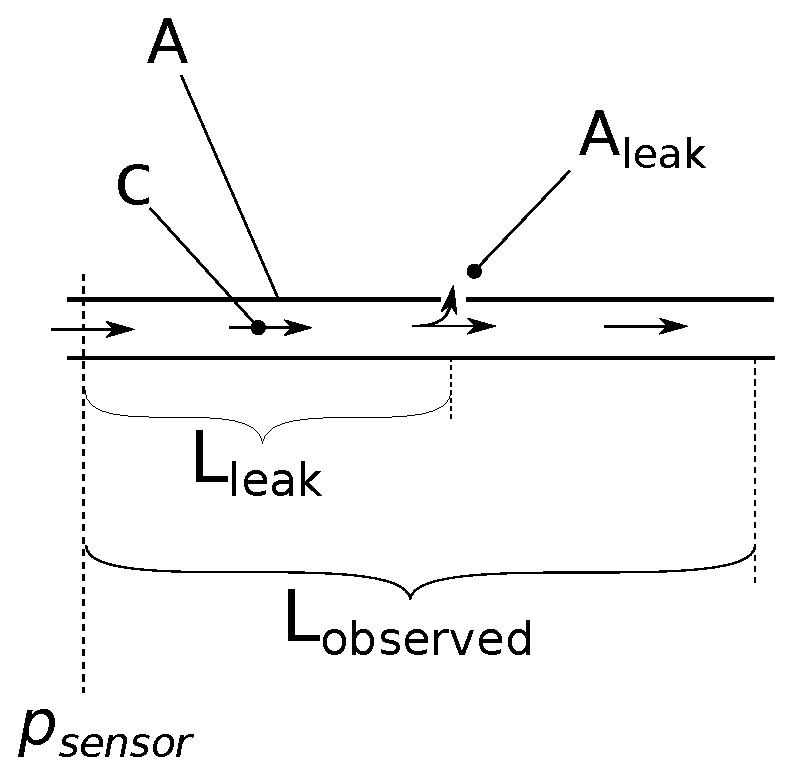
\includegraphics[width=0.9\hsize]{bruch.eps}
\caption{Rohrsegment mit Leckagestelle}
\label{fig:bruch}
\end{figure}

Es handelt sich um einen Rohrabschnitt mit konstanter Querschnittsfläche $A$, durch welchen einem Gas mit nominaler Geschwindigkeit $c$ strömt. Betrachtet wird ein Abschnitt der Länge $L_\mathit{observed}$, bei Lauflänge $L_\mathit{leak}$ ist ein Leck mit einer Querschnittsfläche $A_\mathit{leak}$.

Am Anfang des Segments befindet sich ein Sensor, welcher Eigenschaften der Rohrströmung misst, im gegebenen Fall den statischen Druck $p_\textit{sensor}$.

\subsection{Problem-Parameter}

Das Strömungsmedium ist Methan. Die Fliessgeschwindigkeit $c$ ist $\approx 10\,\mathrm{m/s}$. Der Rohrinnendruck $p$ ist $\approx 60\pm 10\,\mathrm{bar}$. Die Rohrinnentemperatur $T$ ist $\approx 10\,\mathrm{\degree C}$. Die Länge $L_\mathit{observed}$ ist $\approx 500 \ldots 1000 \,\mathrm{m}$.

\subsection{Problem-Frage}

Wie ändert sich die Messung an der Sensor-Stelle, wenn eine Leckagestelle $A_\mathit{leak}$ bzw. $L_\mathit{leak}$ plötzlich auftritt? Lassen sich solche z.B. durch Bauarbeiten verursachten Schäden detektieren durch solche Sensoren detektieren, und wie reagieren die Sensoren im jeweiligen Fall?

\section{Modellierung}

\subsection{Modellierung des Umsystems}

Die Modellierung zielt unter anderem darauf ab, das Umsystem, in diesem Fall die Welt vor und nach dem betrachteten Rohrsegment, realitätsnah nachzubilden.

\begin{figure}[hbp]
\centering
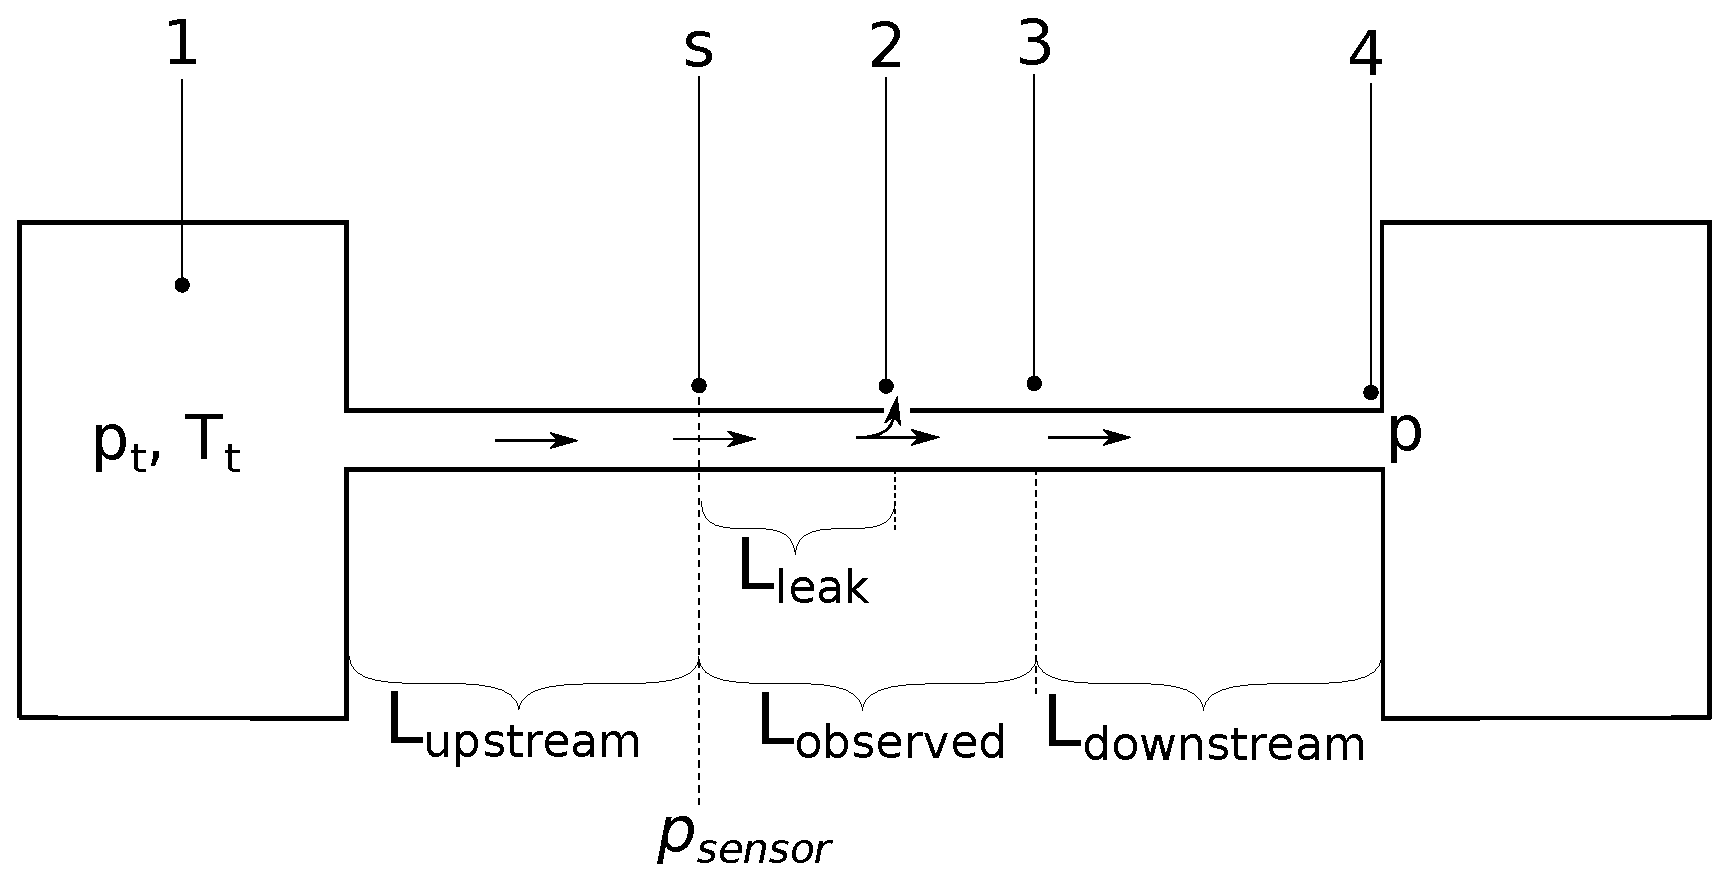
\includegraphics[width=0.9\hsize]{model.eps}
\caption{Modellierung}
\label{fig:model}
\end{figure}

Es wird zwecks Modellierung angenommen, dass sich stromauf und stromab jeweils ein Gascontainer befindet. Es wird angenommen, dass diese Container ein unendliches Volumen haben und ausgeglichen sind\footnote{Damit ist gewährleistet, das weiterer Aus- und Zufluss von Gas den Zustand des Containers nicht verändern, und damit die Randbedingungen beliebig lange stabil sind. Kurzzeitig ist dieses Modell in jedem Fall gültig; falls dieses Modell unzutreffend ist, verringert dies die zeitliche Gültigkeit.}.

Es wir weiterhin hinzugerechnet, dass die Container jeweils über Rohrlängen mit dem betrachteten Rohrsegment verbunden sind, $L_\mathit{upstream}$ in Zufluss- und $L_\mathit{downstream}$ in Abflussrichtung. Mit den jeweiligen Rohrlängen wird Reibung bzw. eine realistische Dämpfung der Systemantwort auf Rohrbruch berücksichtigt.

Folgende Indizes werden in Abb.~\ref{fig:model} verwendet:

\begin{description}
\item[1] ist im Container stromauf, wo das Medium noch in Ruhe (ohne Geschwindigkeit) ist.
\item[s] ist an der Sensor-Stelle, das ist am Ende von $L_\mathit{upstream}$ bzw. am Anfang von $L_\mathit{observed}$
\item[2] ist knapp vor der Bruch- bzw. Leckage-Stelle
\item[3] ist am Ende von $L_\mathit{observed}$ bzw. am Anfang von $L_\mathit{downstream}$
\item[4] ist knapp vor dem Eintritt des Containers stromab bzw. am Ende von $L_\mathit{downstream}$
\end{description}

\subsection{Lösung}

Zur Lösung wird das folgende Netzwerk betrachtet:

\begin{figure}[hbp]
\centering
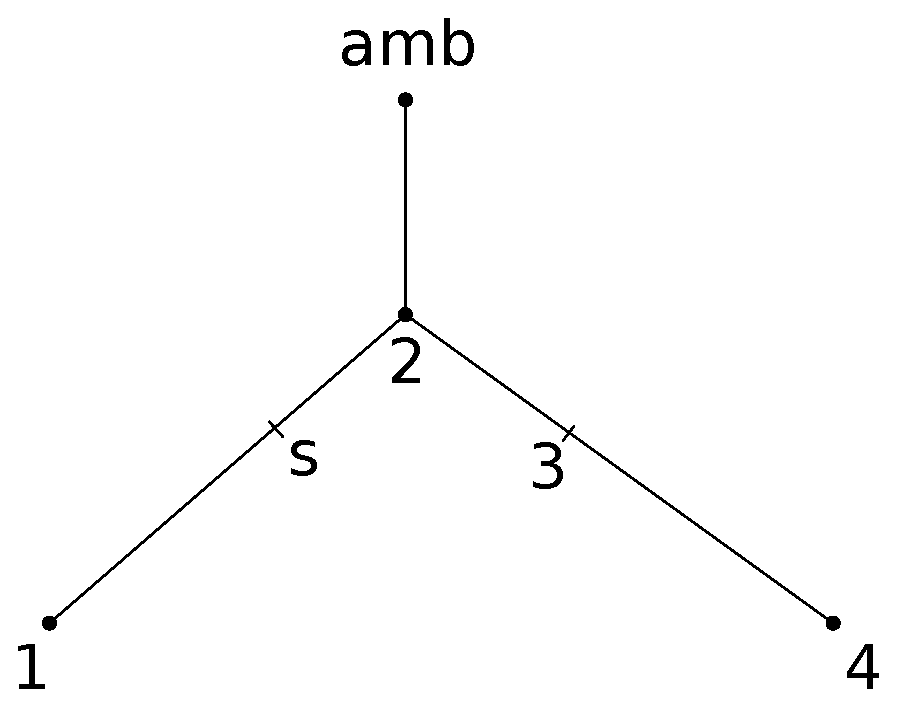
\includegraphics[width=0.9\hsize]{netz.eps}
\caption{Netzwerk}
\label{fig:netz}
\end{figure}

\begin{itemize}
\item die Strecke $\overline{1s}$ ist $L_\mathit{upstream}$
\item die Strecke $\overline{s2}$ ist $L_\mathit{leak}$
\item die Strecke $\overline{s3}$ ist $L_\mathit{observed}$
\item die Strecke $\overline{34}$ ist $L_\mathit{downstream}$
\item von $1$ bis $2$ fliesst der Massenstrom $\dot m_\textit{in}$
\item von $2$ bis $4$ fliesst der Massenstrom $\dot m_\textit{out}$
\item von $2$ nach $\mathit{amb}$ fliesst der Massenstrom $\dot m_\textit{leak}$
\end{itemize}

\subsubsection{Modellparameter}

Die Parameter $L_\mathit{upstream}$ und $L_\mathit{downstream}$ müssen geeignet gewählt werden.


\subsubsection{Systemidentifikation}

Die folgenden Randbedingungen müssen per Systemidentifikation bestimmt werden:

\begin{itemize}
\item an $1$ die Eintrittsrandbedingungen $T_t$ und $p_t$
\item an $4$ die Austrittsrandbedingung $p_4$
\item an $\mathit{amb}$ die Austrittsrandbedingung $p_\mathit{amb}$
\end{itemize}

\subsubsection{Massenstromgleichgewicht}

Es gilt Massenerhaltung:

\begin{equation}
\dot m_\textit{in} = \dot m_\textit{leak} + \dot m_\textit{out} \label{eq:massenerhaltung}
\end{equation}

\subsubsection{Zielgrösse}

Gesucht wird der Druck $p_2$ im Rohr an der Leckage-Stelle. Wenn $p_2$ bekannt ist, lassen sich alle anderen Werte berechnen. $p_2$ lässt sich anhand der Massenerhaltung Gleichung~\ref{eq:massenerhaltung} bestimmen.


\subsection{Hinweise}

\begin{itemize}
\item Machzahlen grösser 1 sind im Rohr und an der Leckagestelle physikalisch nicht möglich, das Gas bewegt sich dort maximal mit Schallgeschwindigkeit; eine numerische Lösung muss Machzahlen grösser 1 ausschliessen
\item Wegen des grossen Druckverhältnisses $p_t$ zu $p_\mathit{amb}$ ist am Leck mit Strömung in Schallgeschwindigkeit zu rechnen
\end{itemize}

\subsection{Einschränkungen}

\begin{itemize}
\item bei hinreichend grossem Leck (ab etwa 5\% des Rohrquerschnitts) würde Rückströmung aus $L_\mathit{downstream}$ auftreten, das ist hier nicht abgedeckt; dann würde sich der Abschnitt $\overline{42}$ so verhalten wie Abschnitt $\overline{12}$; dafür fehlen in der bisherigen Betrachtung noch Eintrittsrandbedingung $T_{t4}$, $p_{t4}$.
\end{itemize}


\appendix

\section{Symbole}

\subsection{Gaskennzahlen}

\begin{tabular}{ l l }
 $R$ & Gaskonstante  \\ 
 $\gamma$ & Isentropenexponent \\  
 $c_p$ & spez. Wärmekapazität bei konst. Druck \\
\end{tabular}

\subsection{Zustandsgrössen}

\begin{tabular}{ l l }
 $T$ & Temperatur \\
 $p$ & Druck \\
 $\rho$ & Dichte \\
\end{tabular}

\subsection{Geometrische Grössen}

\begin{tabular}{ l l }
 $D$ & Durchmesser \\
 $A$ & Querschnittsfläche \\
 $L$ & Länge \\
\end{tabular}

\subsection{Betriebskennzahlen}

\begin{tabular}{ l l }
 $T_t$ & Totaltemperatur \\
 $p_t$ & Totaldruck \\
 $p_{amb}$ & Umgebungsdruck \\
 $\dot m$ & Massenstrom \\
 $c$ & Geschwindigkeit \\
 $\mathit{Ma}$ & Machzahl \\
\end{tabular}

\subsection{Rohrkennzahlen}

\begin{tabular}{ l l }
 $\lambda$ & Rohrreibungszahl \\
 $\zeta$   & Druckverlustbeiwert \\
\end{tabular}


\section{Rohrströmung}

\subsection{Rohrsegmente}

Rohrsegmente sind charakterisiert durch Durchmesser $D$ (oder Kreisquerschnitt $A$) und Länge $L$, siehe Abb.~\ref{fig:leitungssegment}.

Die Wandrauhigkeit wird durch die Rohrreibungszahl $\lambda$ ausgedrückt.

Die Rohrströmung wird durch die Geschwindigkeit $c$ (in $\mathrm{[m/s]}$) bzw. den Massenstrom $\dot m$ (in $\mathrm{[kg/s]}$) beschrieben, in Pfeilrichtung positiv.

\begin{figure}[hbp]
\centering
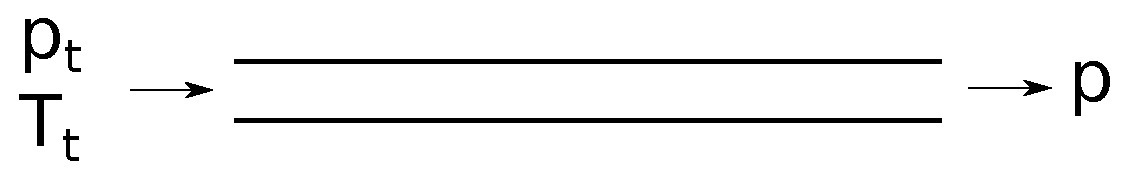
\includegraphics[width=0.9\hsize]{problem.eps}
\caption{Leitungssegment}
\label{fig:leitungssegment}
\end{figure}

\subsection{Randbedingungen}

Für Berechnungen über Rohrsegmente werden in der Strömungsmechanik übliche Grössen für die Randbedingungen verwendet:

Als Randbedingung am Austritt (in Abb.~\ref{fig:leitungssegment} rechts) wird der statische Druck $p$ verwendet, gelegentlich auch als Gegendruck bezeichnet, aber nicht zu verwechseln mit dem Staudruck.

Als Randbedingung am Eintritt (in Abb.~\ref{fig:leitungssegment} links) werden der Totaldruck $p_t$ und die Totaltemperatur $T_t$ verwendet, das entspricht den Zustandsgrössen des Mediums in Ruhe, bei Geschwindigkeit Null.

\subsection{Vernachlässigte Randbedingungen}

Es wird davon ausgegangen, dass die Temperatur von Medium und Umgebung ungefähr gleich ist und deshalb kein signifikanter Wärmeaustausch stattfindet.


\subsection{Idealer Massenstrom}

Der Massenstrom $\dot m$ wird für einen gegebenen Querschnitt $A$ anhand der Totalgrössen $T_t$ und $p_t$ und der lokalen Machzahl $\mathit{Ma}$ berechnet

\begin{equation}
\dot m = A \, \frac{p_t}{\sqrt{T_t}} \sqrt{\frac{\gamma}{R}} \mathit{Ma} \, M^{- \frac{1}{2}\frac{\gamma + 1}{\gamma - 1}}
\end{equation}

Hier ist $M$ die häufig wiederkehrende Hilfsgrösse

\begin{equation}
M = 1 + \frac{\gamma + 1}{2} \mathit{Ma} ^2
\end{equation}

Bei reibungs- und verlustfreier Strömung sind die lokalen 
$T_t$ und $p_t$ gleich den Eintrittsrandbedingungen, unabhängig von der stromauf durchlaufenen Rohrlänge.



\subsection{Ideale Machzahl}

Die Machzahl hängt bei gegebenem $p_t$ nur vom lokalen Druck $p$ ab:

\begin{equation}
\left(\frac{p_t}{p}\right)^\frac{\gamma-1}{\gamma} = 1 + \frac{\gamma + 1}{2} \mathit{Ma} ^2 \label{eq:totaldruckverhaeltnis}
\end{equation}

Wiederum ist bei reibungs- und verlustfreier Strömung der lokale Totaldruck $p_t$ gleich der Eintrittsrandbedingung, unabhängig von der stromauf durchlaufenen Rohrlänge.


\subsection{Reale Strömung}

In realen Rohren bewirkt die Rohrreibung einen Druckabfall $\Delta p$ entlang der Lauflänge:

\begin{equation}
\Delta p = \zeta \rho \frac{c^2}{2}
\end{equation}

mit 

\begin{equation}
\zeta = \lambda \frac{L}{D}
\end{equation}

Der Druckabfall kann näherungsweise berücksichtigt werden, indem ausgehend von der Randbedingung $p_t$ als lokaler, verlustbehafteter Totaldruck $p_t - \Delta p$ angenommen wird, d.h., die Druckverluste $\Delta p$ über einen Rohrabschnitt werden bereits am Eintritt abgezogen.

Damit ergibt sich für den realen Massenstrom $\dot m$:

\begin{equation}
\dot m = A \, \frac{p_t}{\sqrt{T_t}} \sqrt{\frac{\gamma}{R}} \mathit{Ma} \left( M^{ \frac{1}{2}\frac{\gamma + 1}{\gamma - 1}} + \zeta \gamma \frac{\mathit{Ma}^2}{\sqrt{M}} \right) ^{-1}
\end{equation}

Und für den realen, lokalen Druck $p$:

\begin{equation}
p = p_t \left( M^\frac{\gamma}{\gamma-1} + \zeta \gamma \mathit{Ma}^2 \right)^{-1}
\end{equation}

\noindent wobei mit $p_t$ stets die Randbedingung stromauf gemeint ist, nicht der lokale Totaldruck. (Bei gegebenem $p$ und $\mathit{Ma}$ kann der lokale Totaldruck durch Gleichung~\ref{eq:totaldruckverhaeltnis} berechnet werden.)


\section{Grundgleichungen}

Folgende Gleichungen bzw. die damit einhergehenden Annahmen liegen zugrunde und sind zur Herleitung ausreichend:

\begin{eqnarray}
p &=& \rho R T \\
a &=& \sqrt{\gamma R T} \\
\mathit{Ma} &=& c/a \\
c_p T_t &=& c_p T + \frac{c^2}{2} \\
\gamma &=& c_p / c_v \\
R &=& c_p - c_v \\
\frac{T_t}{T} &=& \left( \frac{\rho_t}{\rho} \right)^{\gamma-1} =\,\,\, \left( \frac{p_t}{p} \right)^\frac{\gamma-1}{\gamma} \\
\dot m &=& \rho A c
\end{eqnarray}



\end{document}



